
\chapter{Surface treatments} % Main chapter title

\label{Chapter2.5} % Change X to a consecutive number; for referencing this chapter else where, use \ref{ChapterX}



%-----------------------------------
%	SECTION 3
%-----------------------------------
\section{Oxidation}
Room temperature oxidization is a common way of nanodiamond purification. With different oxidizing temperature, different types of impurities can be removed from the surface of the nanodiamond, ranging from water and physisorbed organic impurities, amourphous carbon, and graphitic shells and ultimate the $sp^{3}$ phase of diamond[T.Gaebel,2010]. After the oxidation, carbonyl and carboxyl groups are formed on the surface[Petrakov,2012]. Several paper have mentioned temperature choices for oxidation aiming at impurity removal. During the master's thesis period, 2 different oxidation has been examined.

\subsection[first Oxidation]{first Oxidation}
As reported, it is possible to achieve the removal of $sp^{2}$ carbon without any oxidation on $sp^{3}$ carbon via aerobic oxidation with temperature between 375$^{o}C$ and 450$^{o}C$. With temperature lower than 500$^{o}C$, the size reducing rate of nanodiamond is lower than 1nm/h. As our first treatment, we carried out a two step oxidation on sample 1508 and 1509, to achieve the complete removal of graphitic defect on the surface and light oxidation on the surface. Sample 1508 was spin coated with nanodiamond batch2, sample 1509 was spin coated with nanodiamond batch1.

The aerobatic oxidation is carried out in a tube furnace and it is done with the help of Markus Mohr. The tube furnace consists of a glass tube connected to the room atmosphere and heating coils around the glass tube. The glass tube can be slide in or out of the heating coils. We put our sample inside a ceramic sample holder and put the holder into the glass tube carefully, after the temperature has been raised to 460$^{o}C$, the glass tube was slide into the heating coils. The sample was oxidized at 460$^{o}C$ for 90min,then 480$^{o}C$ for 40min. After the Oxidation, the glass tube was slide out and the sample stayed inside the tube until it reached room temperature.

Before the oxidation, the samples was first mapped with a room temperature setup that resembles fig. 2.4, but without vaccum pump and cryostat. To make a map of SiV$^{-}$ containing points of interest, it was first taken, a scan with green laser while the fluorescence was recorded by APD, which offers us a confocal microscopy image of the sample, then the photoluminescnce spectra of the bright spots were taken, coordinates of those ones with a sharp peak at 737nm saved as points of interests for the reference of further examine.

\begin{figure}[h]
\centering
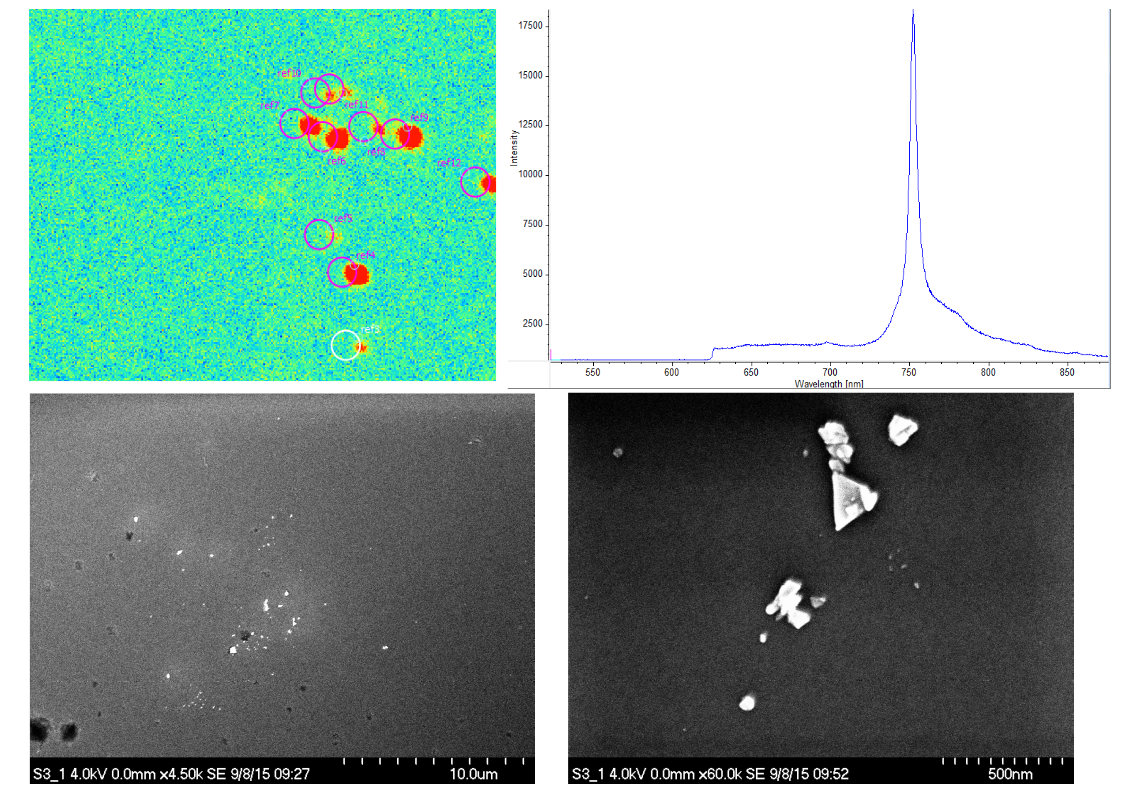
\includegraphics[width=1\linewidth]{Figures/pic/RTPL}
\caption{A)confocal image of a region of interest. The bright spots with circle markers are points of interest. B)Room temperature spectrum of a poi recorded by spectrometer. C)the roi in SEM. D)ref10 and 11 in SEM.}
\label{fig:2015-09-07-ow-capture-20150907151210-744-1}
\end{figure}

Once the map was acquired, we bring the samples to the electron microscope center and observed the regions of interest with SEM. SEM showed that, sample1508 contains more big single crystals that are larger than 300nm and clusters, while sample 1509 contains more single crystal with under 200nm sizes. This proved that the size selection via centrifuging has worked.
 
The samples was then attached to an cold finger and the placed inside the cryostat, after UHV condition has been achieved, the helium transfer was started, which would brought the temperature of the sample down to 4.8K. Most of the mapped pois are refound. Excitation with 532nm green laser double checked the existence of SiV. After the confirmation, it has been tried to carry out a resonance excitation with Titan Sapphire laser, when observing a few points of interest next to marker 5A in sample1509, it was noticed that while scanning the red laser across the line with the help of very low amount of 532nm for repopulation, a spectral diffusion of 6GHz in 15Min has been observed. To exclude the possibility of instrumental error, PLE has been operated on the bulk diamond sample with also SiV inside, where no spectral diffusio has been observed(Fig. 3.2). It has also been noticed that the increase of green laser power can cause more severe spectral drift/jump. In a case when the power green laser is brought up for a better refocus, the line has shifted totally out of the range of the spectra scan, and didn't recover in 10min. This observation brought difficulty in the measurement of orbital T1, since we always need to initialize the obital states with green laser, and this spectral diffusion that is related to the application of green laser can result in the fail of hitting the resonant wavelength, since it is technically difficult to refind the line and adjust the wavelength of the resonance laser coordinately. 

\begin{figure}[h]
\centering
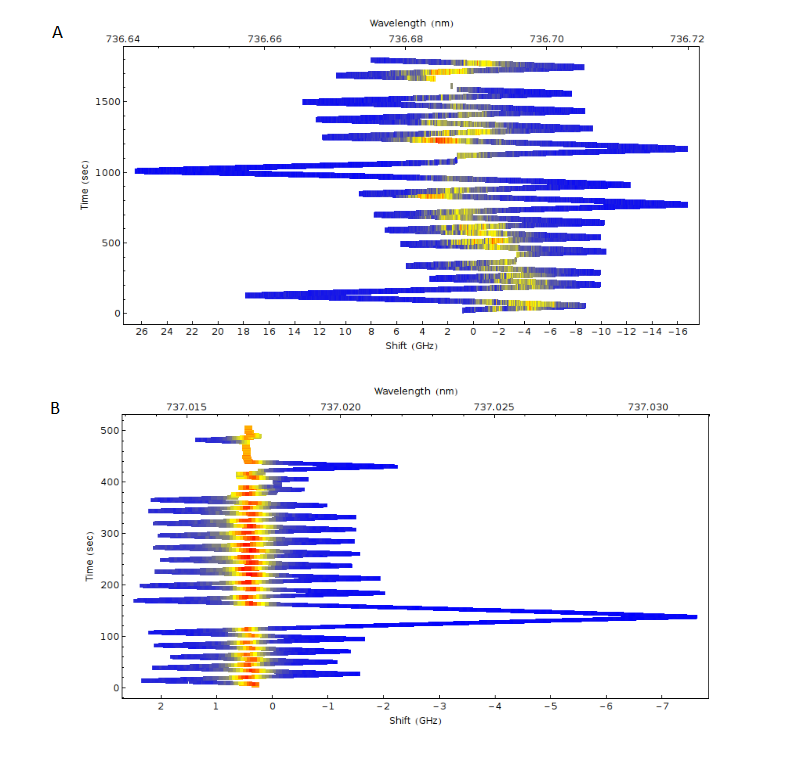
\includegraphics[width=0.7\linewidth]{Figures/pic/PLE}
\caption{PLE scan over time on A) ref5A$\textunderscore$014 from sample1509 and B) a SiV$^{-}$ site from bulk diamond sample 33b. No significant spectral diffusion been found in bulk diamond sample, which exclude the possibility of instrumental error.}
\label{fig:ple}
\end{figure}

After the obeservation above, we want to study more about this spectral diffusion behaviour that is associated with the green laser. We noticed that the sudden jump/diffusion when more green power is applied can be larger than 20GHz, maybe it is easier to track the movement of the lines with the high resolution grating of spectrometer than with PLE.

To observe the diffusion with a spectrometer, we introduced time-resolved photoluminescen spectrum, which has been described in last chapter. Due to the technical problem, our motorized sample stage can not move ideally in the vertical direction anymore, which has limited our region of observation. This time we refound the ROI around the marker 4C. And recorded the time-resolved spectrum. A session is set to be 60 spectra taken consecutively. At first, to feel the long term diffusing better, 3 sessions, with a refocus after each, are undergone for each points of interests. Since line diffusion in PLE gets wider when raising the green laser power, we excite the sample with 500uW power in front of the objective lens to obtain more diffusion. As a result, line diffusion up to 1nm has been observed.Sequentially we decrease the input power to examine the power dependency of spectral

Taking the samples out of the furnace, we noticed that the surfaces of the samples turned very dirty. It is yet not clear, what the contaminations are, are they intrinsic or are they extrinsic. A possible explanation is that, the contamination comes from the glass tube of tube furnace, that the residues of previous treatments has attached to the inner surface of the tube and evaporized again, depositing on the surface of our sample. Further improvement of oxidation operation has been done in our second oxidation test, and will be mentioned in the next part of the thesis.
\begin{figure}[h]
\centering
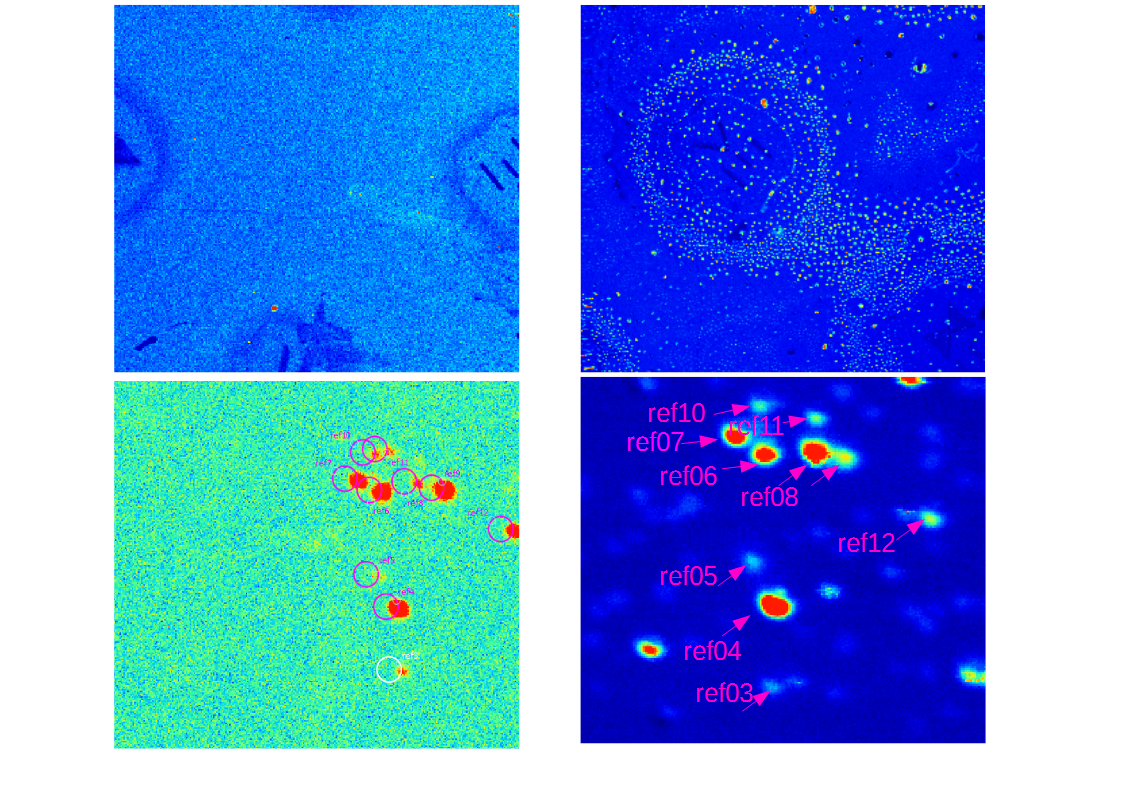
\includegraphics[width=0.7\linewidth]{Figures/pic/oxidation}
\caption{A) region of interest next to marker 3C of sample 1508 before oxidation B)the same region of interest after oxidation C) Points of interest from the ROI before oxidation D)points of interest after oxidation}
\label{fig:oxidation}
\end{figure}

After the oxidation, both of the samples showed very bright background. In sample 1508, large amount of bright spots around the markers has been found. They are not SiV or NV, and will bleach away very fast once been focused on.

I couldn't re-find any marker from sample 1509 due to the large amount of fluorescence from the surface. For sample 1508, the region of interest next to marker 3C was still visible, despite all the disturbing bright spot next to it.

Sample 1509(substrate 207) was then acid cleaned, at the same time sample 1508 was moved into the cryostat, time resolved spectra were recorded. After the oxidation, we learned that the beam polarisation is not conserved within the photonic fibre, so that a polarising beam splitter and a liquid crystal noise eater was added after the fibre to obtain steadily vertically polarised beam. Using the same method as before oxidation, time-resolved PL spectra was recorded.

\subsection[Second Oxidation]{second Oxidation}

The surface function groups play very important role regarding the surface charging state. It is interested to observe, the spectral behaviour of SiV in nanodiamonds, when the surface is initialized the same as bulk diamond. As reported in [Wolcott 2014], after 2 hours of aerobatic oxidation at $575^{o}C$, the surface structure of HPHT NDs is very similar to bulk single crystals where hydroxyl and possibly ethers are the dominant functional groups. It is also interesting, since the elevated oxidation temperature can reduce the size of nanodiamond, to observe the behaviour change as the SiVs will be even closer to the surface after oxidation. Sample 1510 was prepared for this treatment, nanodiamond from batch1 was spin coated on the substrate186$\textunderscore$1 with method IV.

We tried to spin coat substrate 207 at the same time, but failed. The droplet of liquid refuse to spread over the surface while spinning, we suspect the surface of substrate has been damaged in our last oxidation session, which may result in a higher surface roughness that leads to poor wettability.

Taking the experiences of last oxidation into consideration. This time we introduced inert gas (helium) flow to flush away the potential contaminations during the cooling process. This can also prevent the result to be affected by the humidity of the air.
We found out the extinction rate of polarising beam spliter was not ideal for 532nm, so this time we used a Clan Thompson polarisation filter instead.

As mentioned, the polarisation of the beam was not fixed in the measurement before the first oxidation, and while comparing the before and after oxidation spectra, we noticed that, even when the 2 sets of spectra are from the same poi, the spectra pattern can be very different. This made me wonder, if the polarisation of excitation beam has anything to do with the spectral diffusion. To figure this out, we measured the time-resolved PL spectra on 3 pois with different excitation beam polarisation at 4.7K.

The excitation polarisation pattern of other pois are also recorded, but due to low time and Helium budget, it was not affordable to record time resolved excitation polarisation for each of them. Time-resolved PL was later recorded at 20K.

After the oxidation, it was noticed that the sample looks much cleaner than last time. The confocal observation confirmed that, no bright dots like the ones from sample1508 has been seen. The increase of background fluorescence was observed again. Cold spectra showed the existence of GR1 center everywhere.

\begin{figure}[h]
\centering
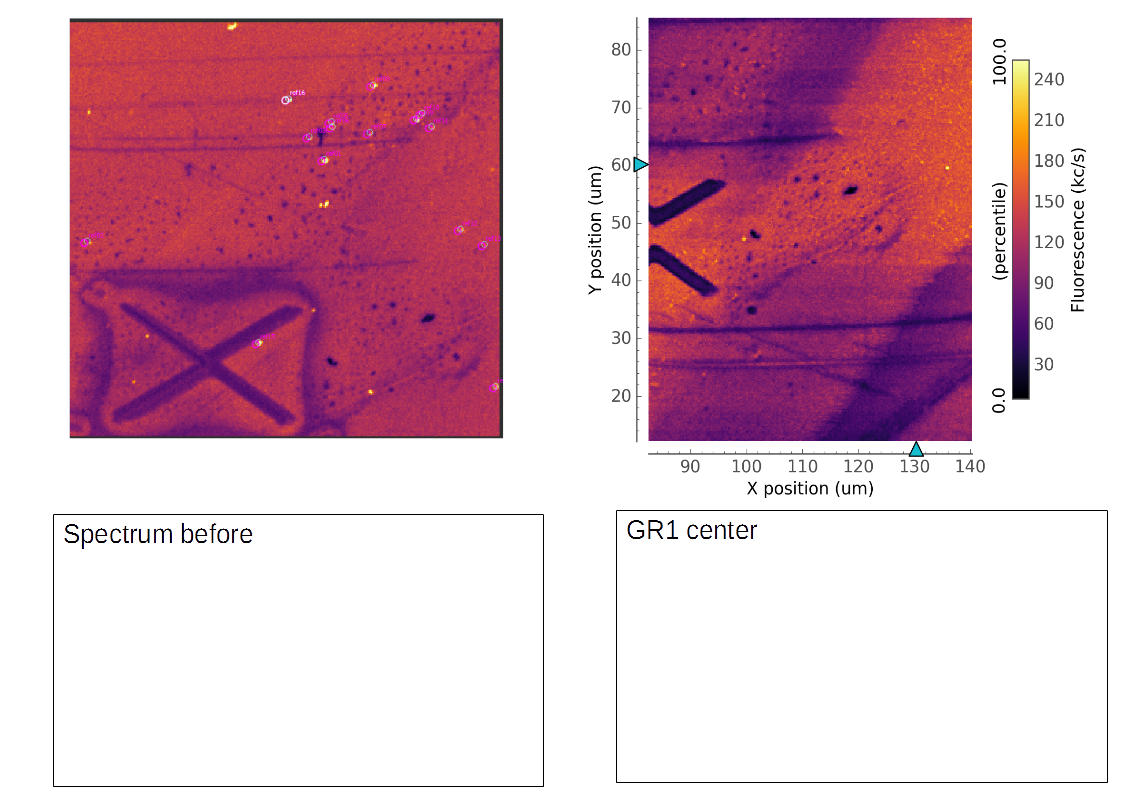
\includegraphics[width=0.7\linewidth]{Figures/pic/afteroxidation2}
\caption{A) roi before oxidation, pois are mapped.B)roi after oxidation, strong background fluorescence, can't find pois.C)spectrum of poi before, no strong Gr1.D)Spectrum after oxidation, strong GR1 center everywhere.}
\label{fig:wp20160921204221proli}
\end{figure}

I noticed the intensity of GR1 fluorescence is stronger around the FIB made markers. As GR1 centre is a isolated vacancy inside diamond, it is reasonable to suspect that, the impact of focused ion beam may have caused serial collision and collision-induced dislocation inside diamond, resulting in the formation of GR1 centre. The fact that the intensity of GR1 centre is higher after the oxidation can also be explained by this theory, since the cross section is usually of the shape of a droplet, which is larger a few nm beneath the surface that on the surface.

%----------------------------------------------------------------------------------------
%	SECTION 4
%----------------------------------------------------------------------------------------

\section[H termination]{H termination}
As we discussed before, the origin of the band bending is that, the chemical potential of the surface and the bulk region need to match each other, while this adjustment changes the density of charges inside the diamond, it stimulates the generation of space charge, which need to be compensated by the surface charge that is compatible with the shift of the Fermi level from the charge neutrality level (CNL) of the surface state system. The hydrogenate of the diamond surface covers the surface with an atomic layer of $C^{\text{-}} H^{+}$ dipole, which lowers the surface potential, switches the surface from PEA to NEA. I has been experimentally proved that Hydrogenated n-doped diamond has flatter band bending than dehydrogenated ones.[Diederich,1998] 



\FloatBarrier
\begin{figure}[h]
\centering
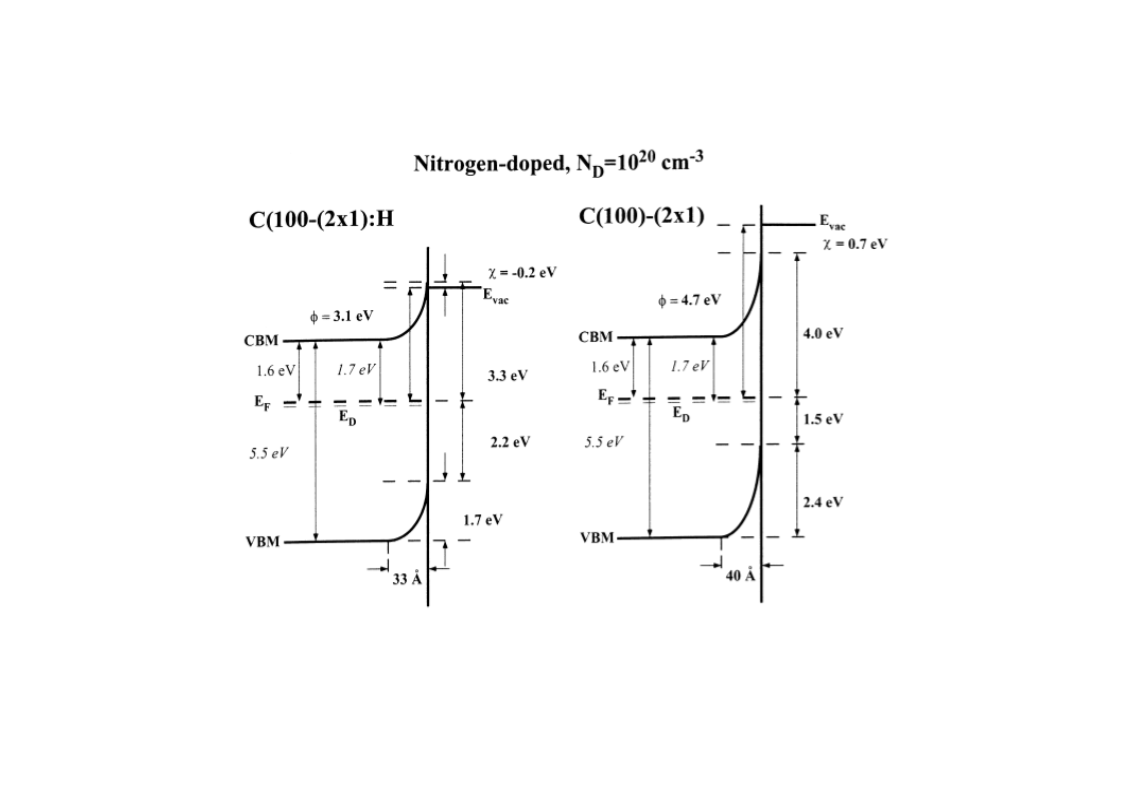
\includegraphics[width=0.7\linewidth]{Figures/pic/Htermination}
\caption{Band structure of N-doped diamond, due to the shift of surface chemical potential, Hydrogenated diamond has flatter band bending than dehydrogenated diamond.[Diederich,1998]}
\label{fig:wp20160921210516proli}
\end{figure}
\FloatBarrier

The surface termination is carried out in a microwave plasma reactor. This is operated by Dr. Christian Osterkamp. We used the same parameters for bulk diamond, (ASK OSCHDI). In [Yeap, 2009], the reaction lasted 60min to maximize the coverage, in our case, considering the low density of nanodiamond on the substrate, we applied the same amount of time as bulk diamond, as the nanodiamond can already be 'dipped' into the plasma thoroughly. The sample that has been used is sample 1512. Sample 1512 was produced by spin coating nanodiamond batch1 on the substrate 186$\textunderscore$2, with method IV.

To prevent introducing contamination into the plasma reactor, no characterisation has been done before the termination. The plasma reactor has the similar vacuum system as a conventional electron microscope, the sample was first put into a pre-vacuum chamber then send into the reaction chamber. The shape of the plasma is controlled by a quartz waveguide. 

After the termination, we put the sample directly into the cryostat, very high density of SiV has been found and marked. It has been recorded as before, the excitation polarisation pattern and the time-resolved PL spectra.
\begin{figure}[h]
\centering
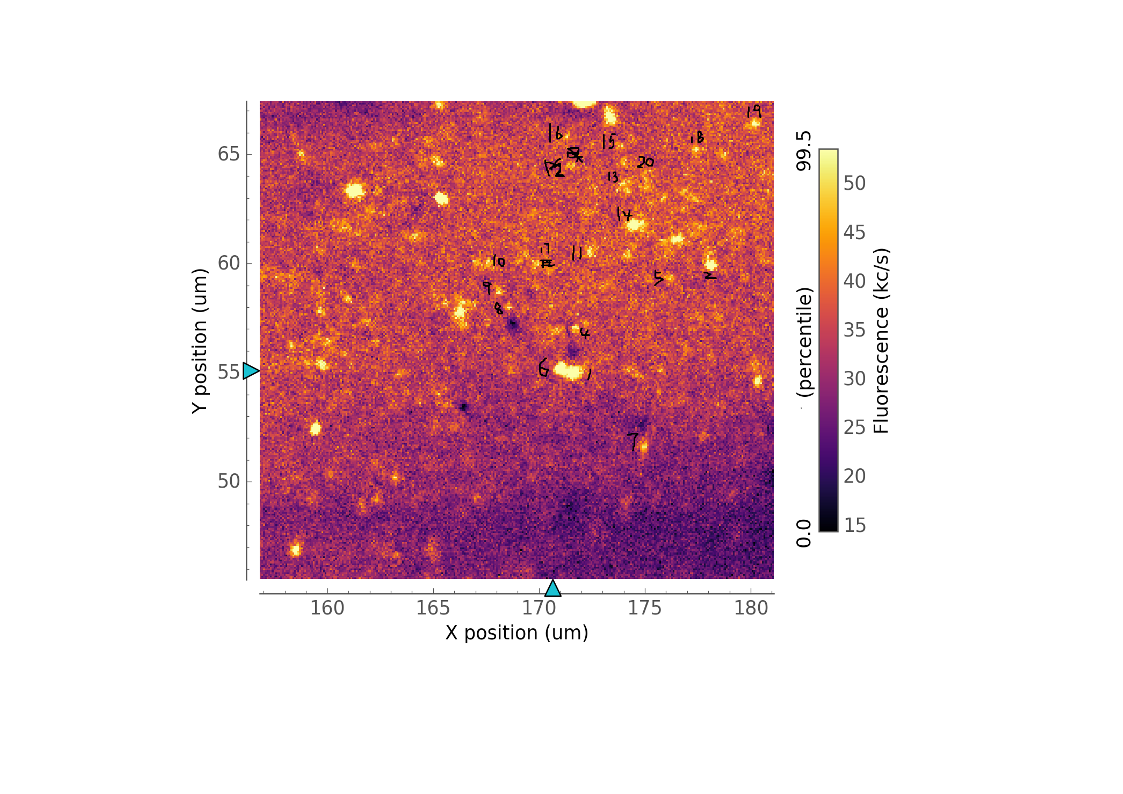
\includegraphics[width=0.7\linewidth]{Figures/pic/hmap}
\caption{Very high density of SiV has been found in sample 1512}
\label{fig:hmap}
\end{figure}

